\chapter{业务对象及相互关系}
\section{概述}
本系统的主要业务模块分为房源管理,新闻管理,用户权限管理,系统管理,技术模块分为前端技术和后端技术,技术栈为:
\begin{itemize}
    \item 后端技术: SpringCloud + SpringSecurity + Nacos + OpenFeign + Spring Gateway + Mybatis-plus + MySQL
    \item 前端技术: 
\end{itemize}
\section{业务概念一览}
本系统的模块可以详细分为用户、角色、权限、房源、新闻、信息、举报、审核、日志、通讯这十个模块。下图为这几个模块的关系类图。
\begin{figure}[htbp]
    \centering
    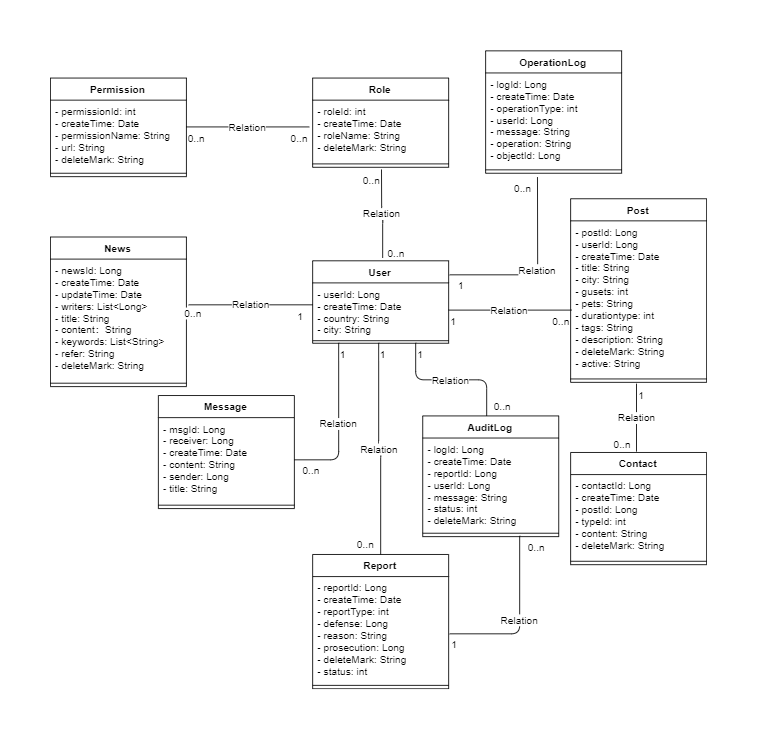
\includegraphics[width=1\textwidth]{ch5/AkraineHelper.png}
    \caption{总类图}\label{fig:AkraineHelper}
    \vspace{\baselineskip} % 表示图与正文空一行
\end{figure}
\section{登录}
登录是个较为复杂的模块,因为他需要认证用户信息,生成用户登录凭证,还需要将用户的权限信息存入缓存中以便后续的鉴权工作。

登录模块使用了SpringSecurity架构,其中我们自定义了登陆用户信息,还有一些相关过滤器,同时我们使用了SpEL语言在AuthCheckeService中重定义了系统的鉴权规则,使得系统动态
匹配用户权限信息。同时用户密码的加密,以及登陆凭证的生成都是根据项目实际情况自行定义的,其类图关系如下。
\begin{figure}[htbp]
    \centering
    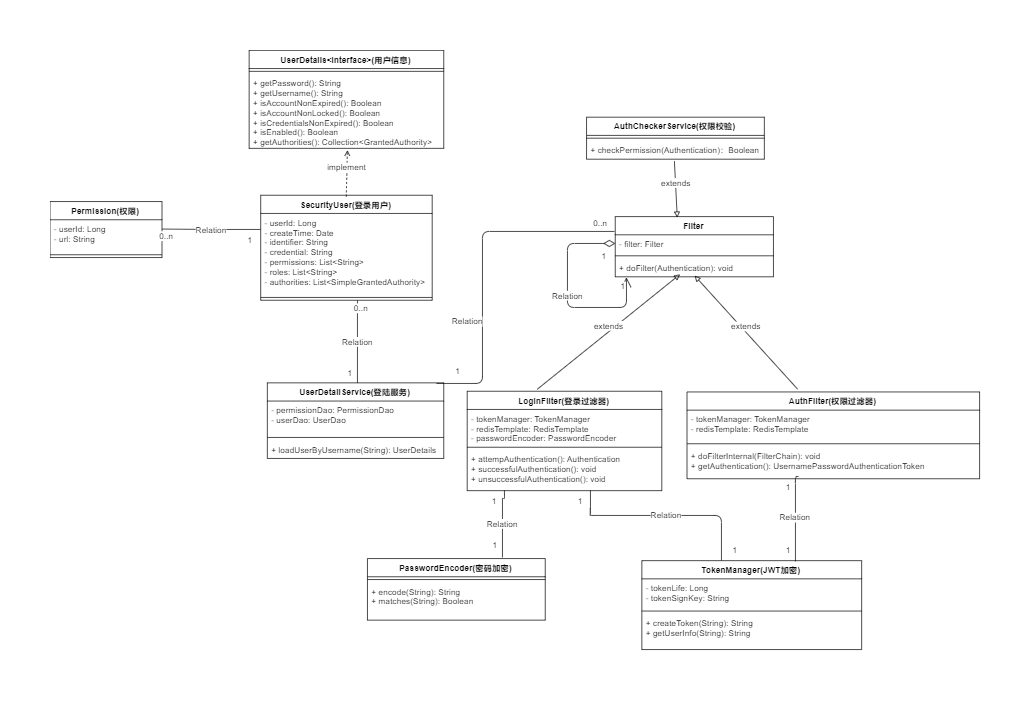
\includegraphics[width=1\textwidth]{ch5/Authentication.png}
    \caption{登录}\label{fig:Authentication}
    \vspace{\baselineskip} % 表示图与正文空一行
\end{figure}
\section{发布房源}
房源发布主要为屋主的操作,该模块要求屋主填写填写房源基本信息,包括房源地址,容纳人数,是否允许宠物等,还需要屋主留下联系方式,难民可以根据联系方式
自行去联系屋主。涉及到的实体类有用户类(User),帖子类(Post),联系方式(Contact),标签(Tag)。具体的方法都在PostController中进行调用。
\begin{figure}[htbp]
    \centering
    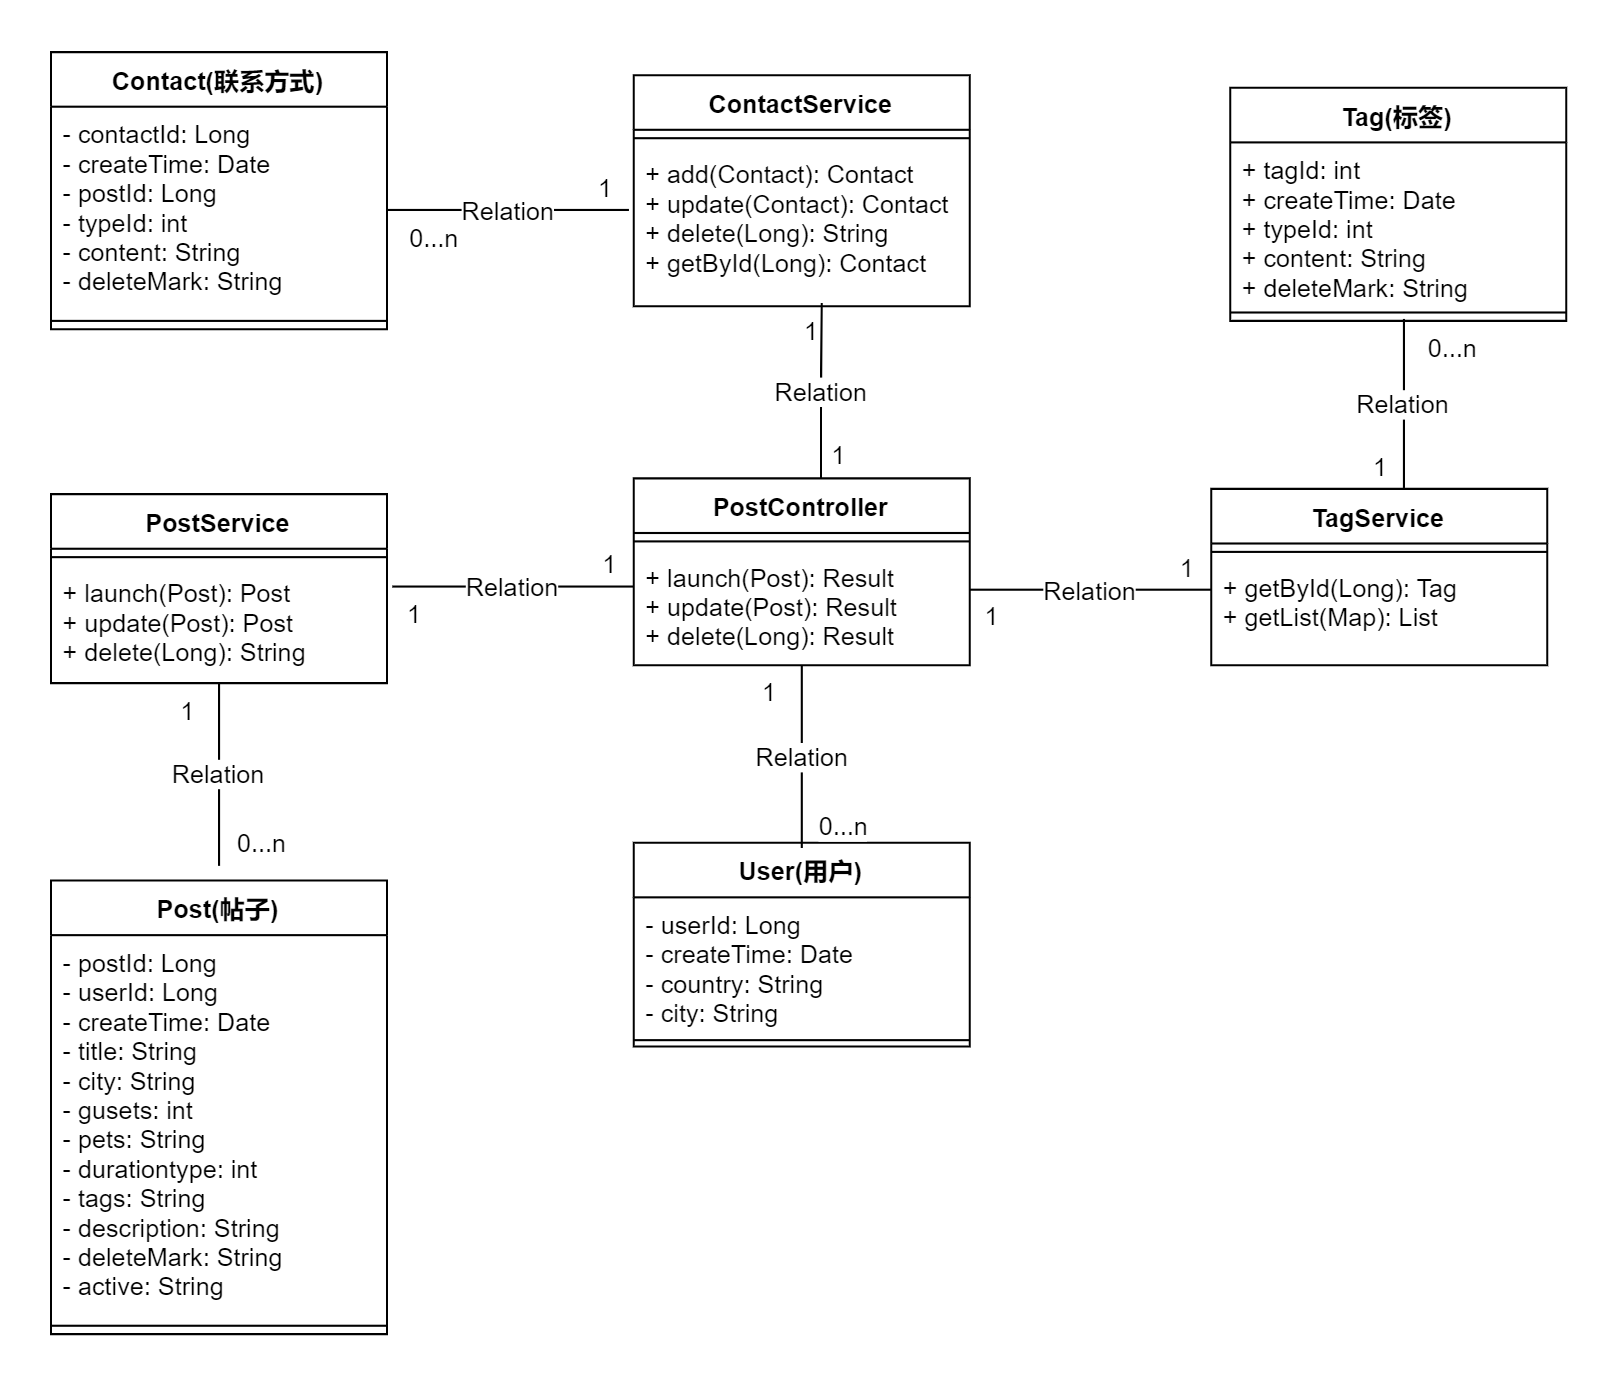
\includegraphics[width=1\textwidth]{ch5/LaunchPost.png}
    \caption{发布房源}\label{fig:LaunchPost}
    \vspace{\baselineskip} % 表示图与正文空一行
\end{figure}
\section{修改房源}
屋主可以查看自己发布的房源,然后进行修改,比如添加删除标签,修改联系方式等等,具体的方法还是在PostController中调用。
\begin{figure}[htbp]
    \centering
    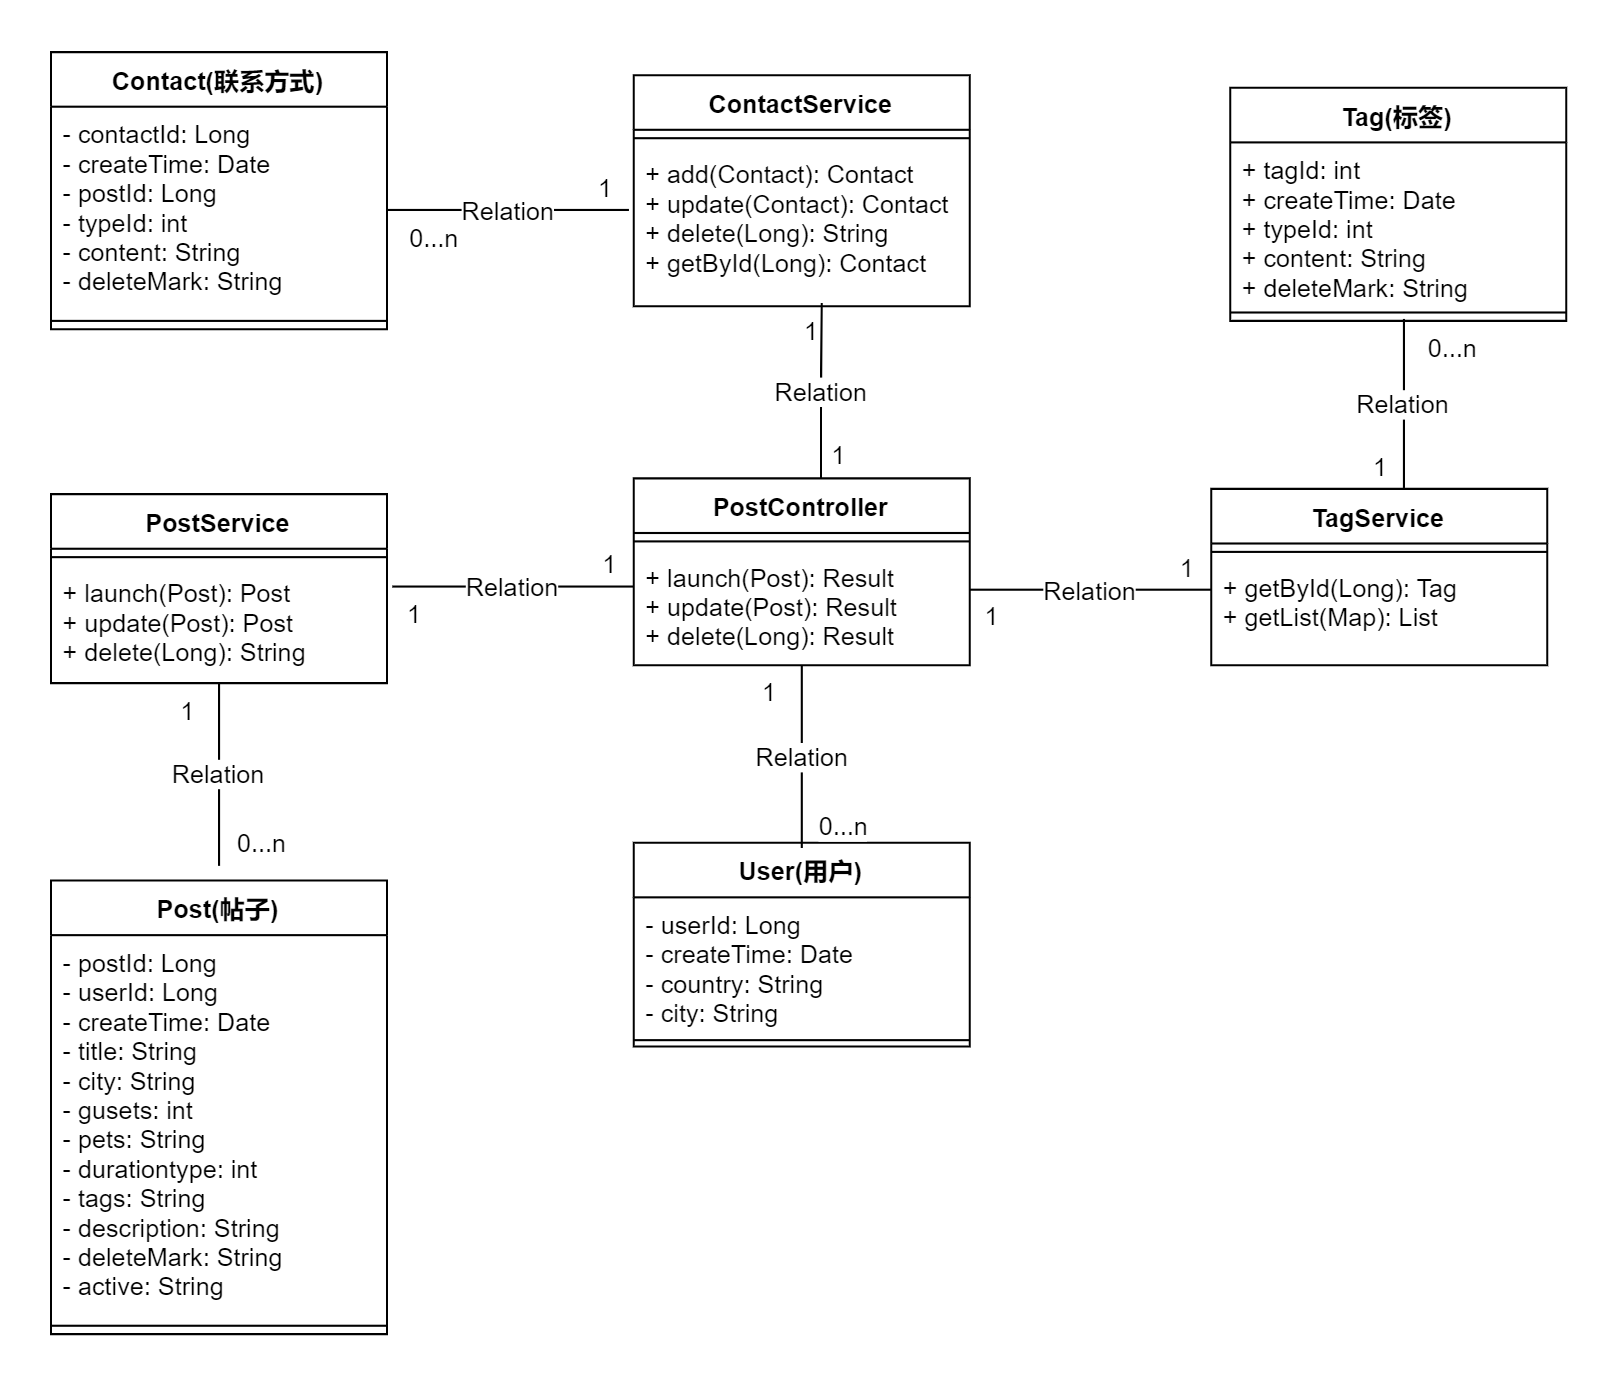
\includegraphics[width=1\textwidth]{ch5/LaunchPost.png}
    \caption{修改房源}\label{fig:UpdatePost}
    \vspace{\baselineskip} % 表示图与正文空一行
\end{figure}
\section{删除房源}
屋主可以查看自己发布的房源,然后进行删除操作,就可以将发布过的房源不再显示。
\begin{figure}[htbp]
    \centering
    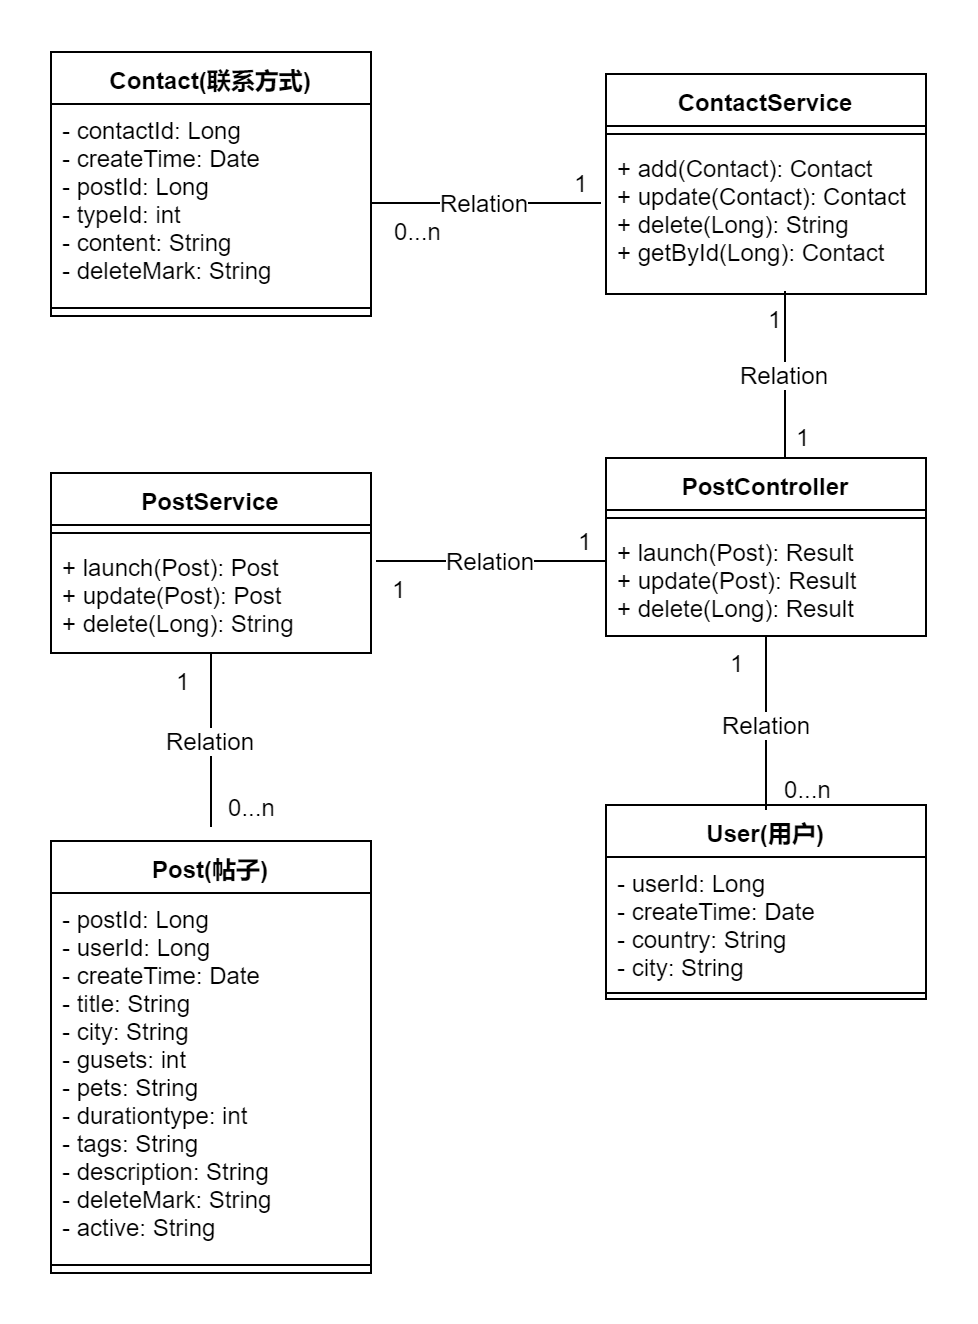
\includegraphics[width=1\textwidth]{ch5/DeletePost.jpg}
    \caption{删除房源}\label{fig:DeletePost}
    \vspace{\baselineskip} % 表示图与正文空一行
\end{figure}
\section{发布新闻}
发布新闻主要为编辑者的操作,该模块要求编辑者填写新闻的详细信息,包括新闻标题,新闻内容,关键词等,如果是引用的别的网站的新闻则需要注明引用链接,
新闻模块是所有用户均能观看。新闻需要进行审核才能发布。涉及到的实体类有用户类(User),新闻类(News),审核类(AuditLog)。具体方法都在NewsController中进行调用。
\begin{figure}[htbp]
    \centering
    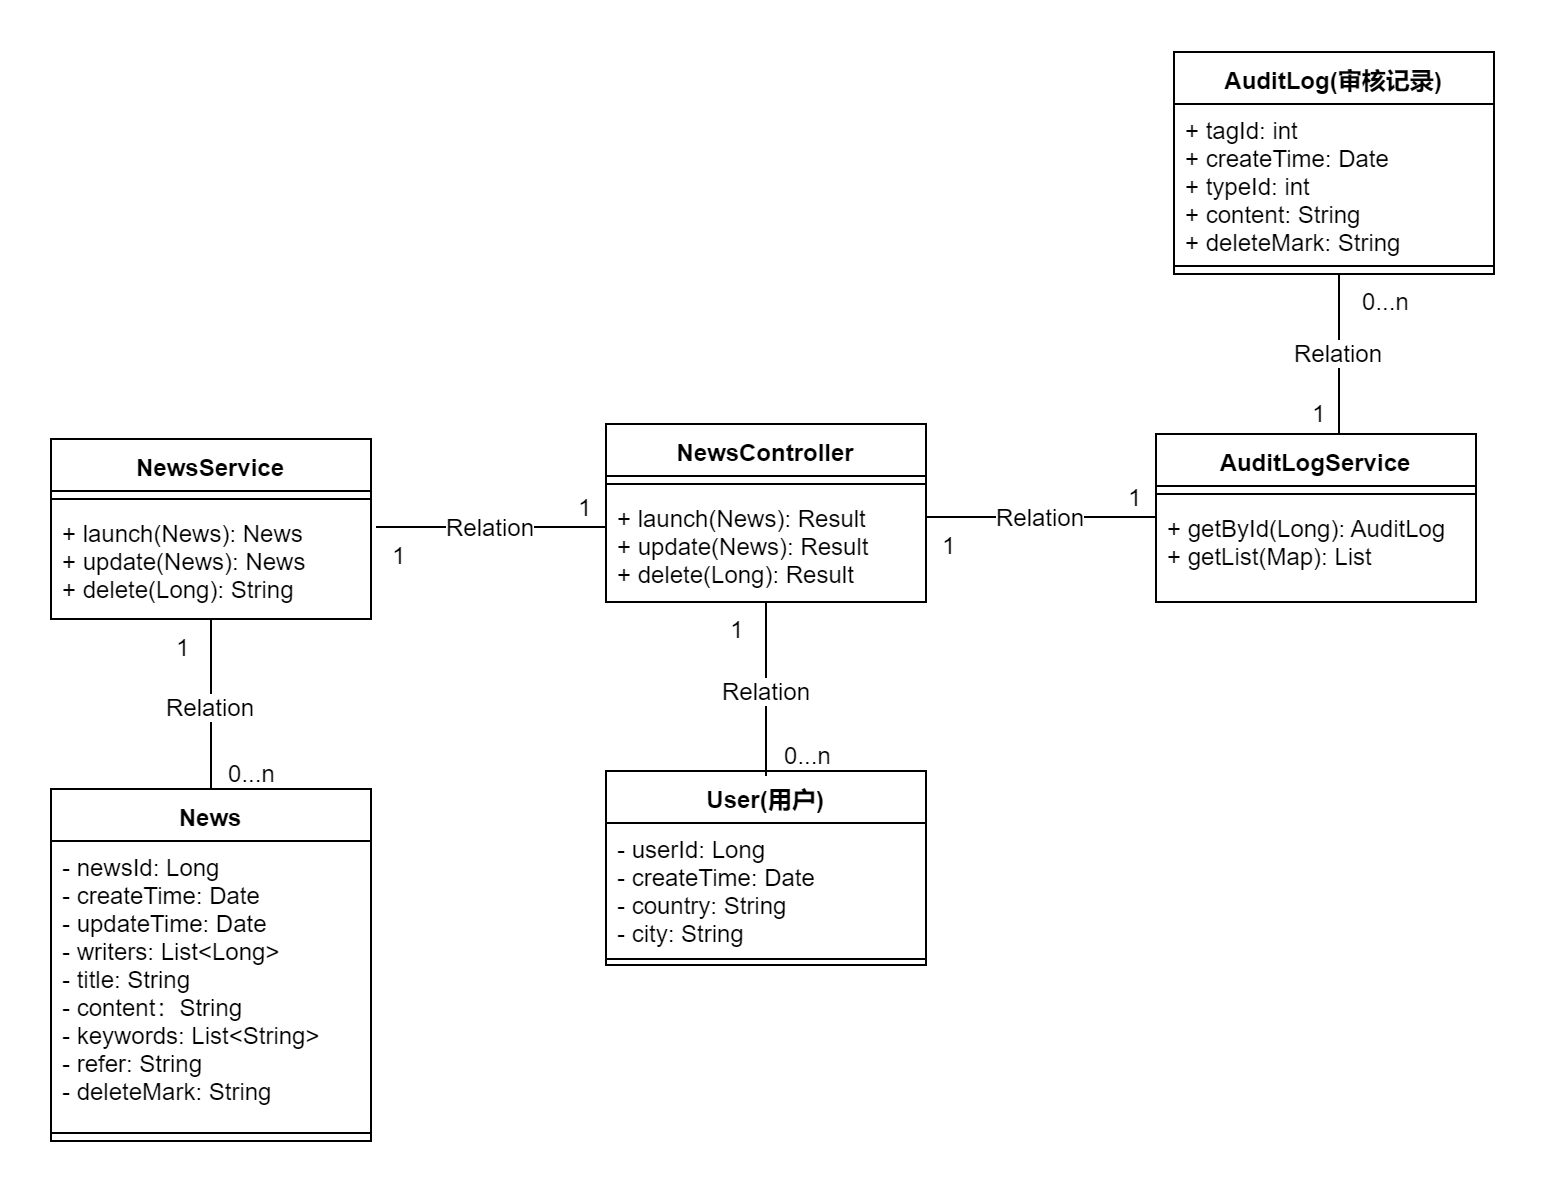
\includegraphics[width=1\textwidth]{ch5/LaunchNews.jpg}
    \caption{发布新闻}\label{fig:LaunchNews}
    \vspace{\baselineskip} % 表示图与正文空一行
\end{figure}
\section{修改新闻}
编辑者可以查看自己发布的新闻,然后进行修改,比如修改内容,修改标题等等,修改后需要审核才能发布。具体的方法还是在NewsController中调用。
\begin{figure}[htbp]
    \centering
    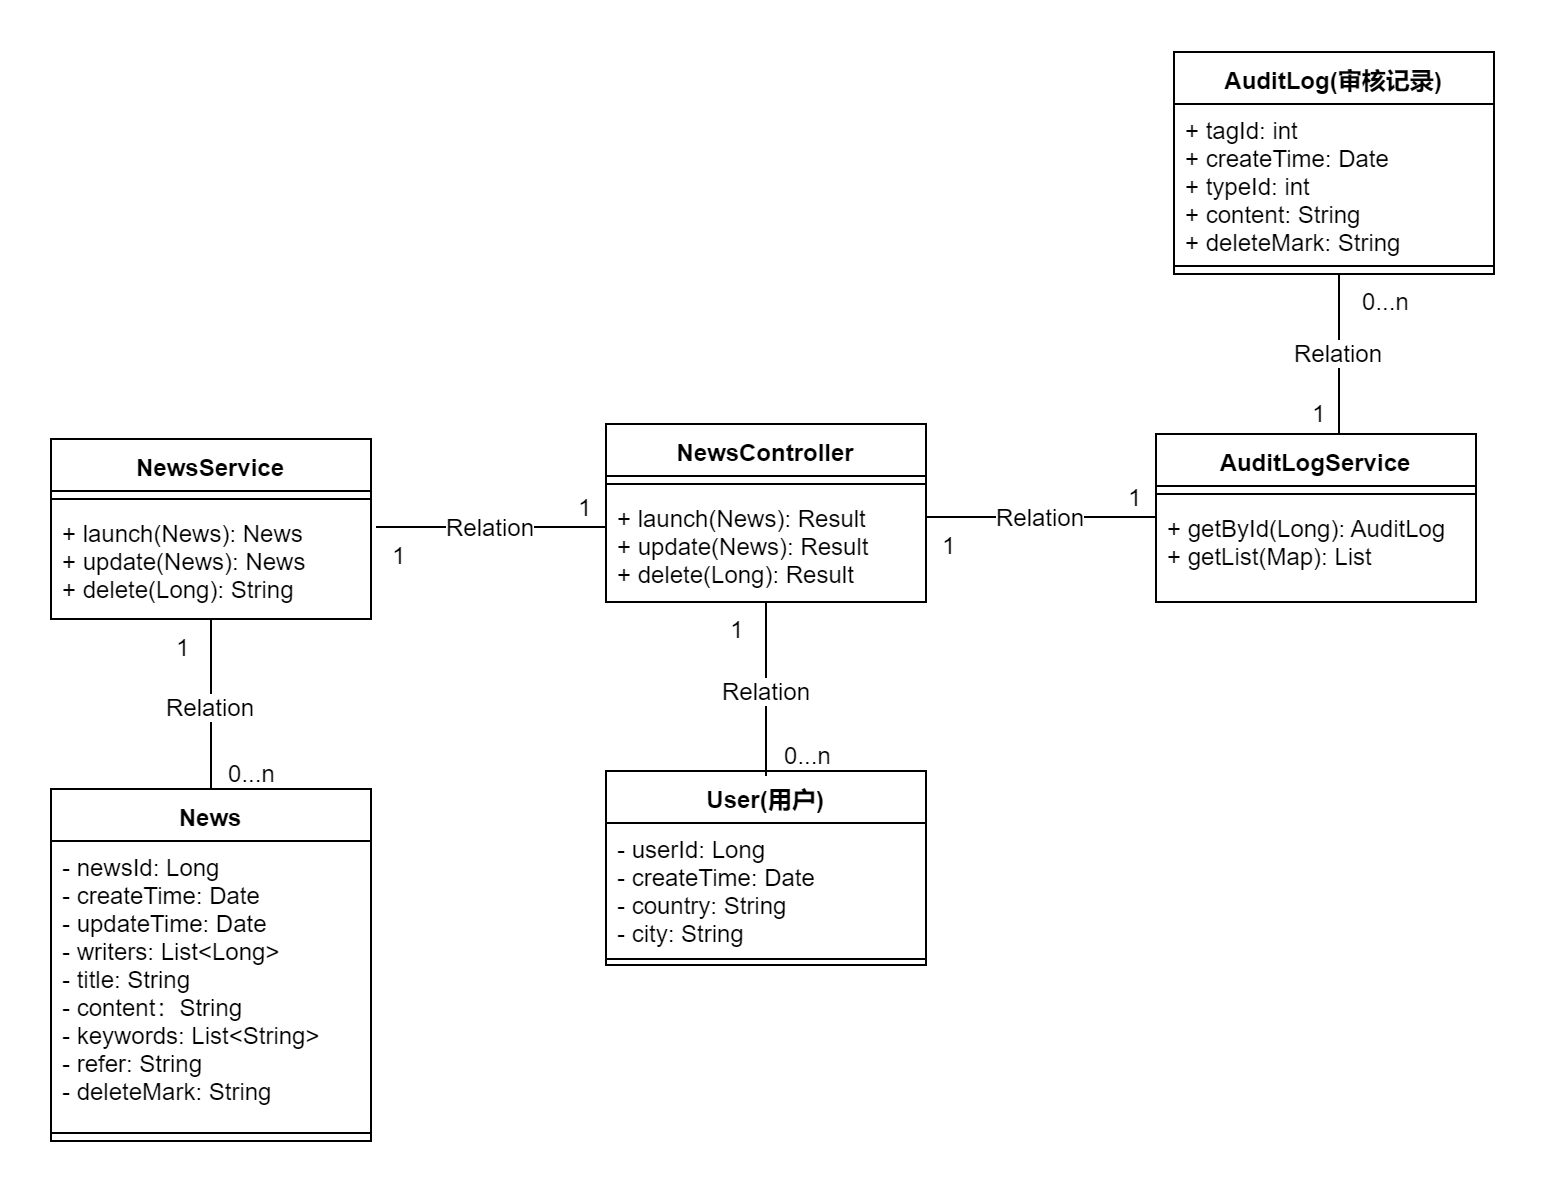
\includegraphics[width=1\textwidth]{ch5/LaunchNews.jpg}
    \caption{修改新闻}\label{fig:UpdateNews}
    \vspace{\baselineskip} % 表示图与正文空一行
\end{figure}
\section{删除新闻}
管理员可以查看发布的新闻,然后删除操作,具体的方法是在NewsController中调用。
\begin{figure}[htbp]
    \centering
    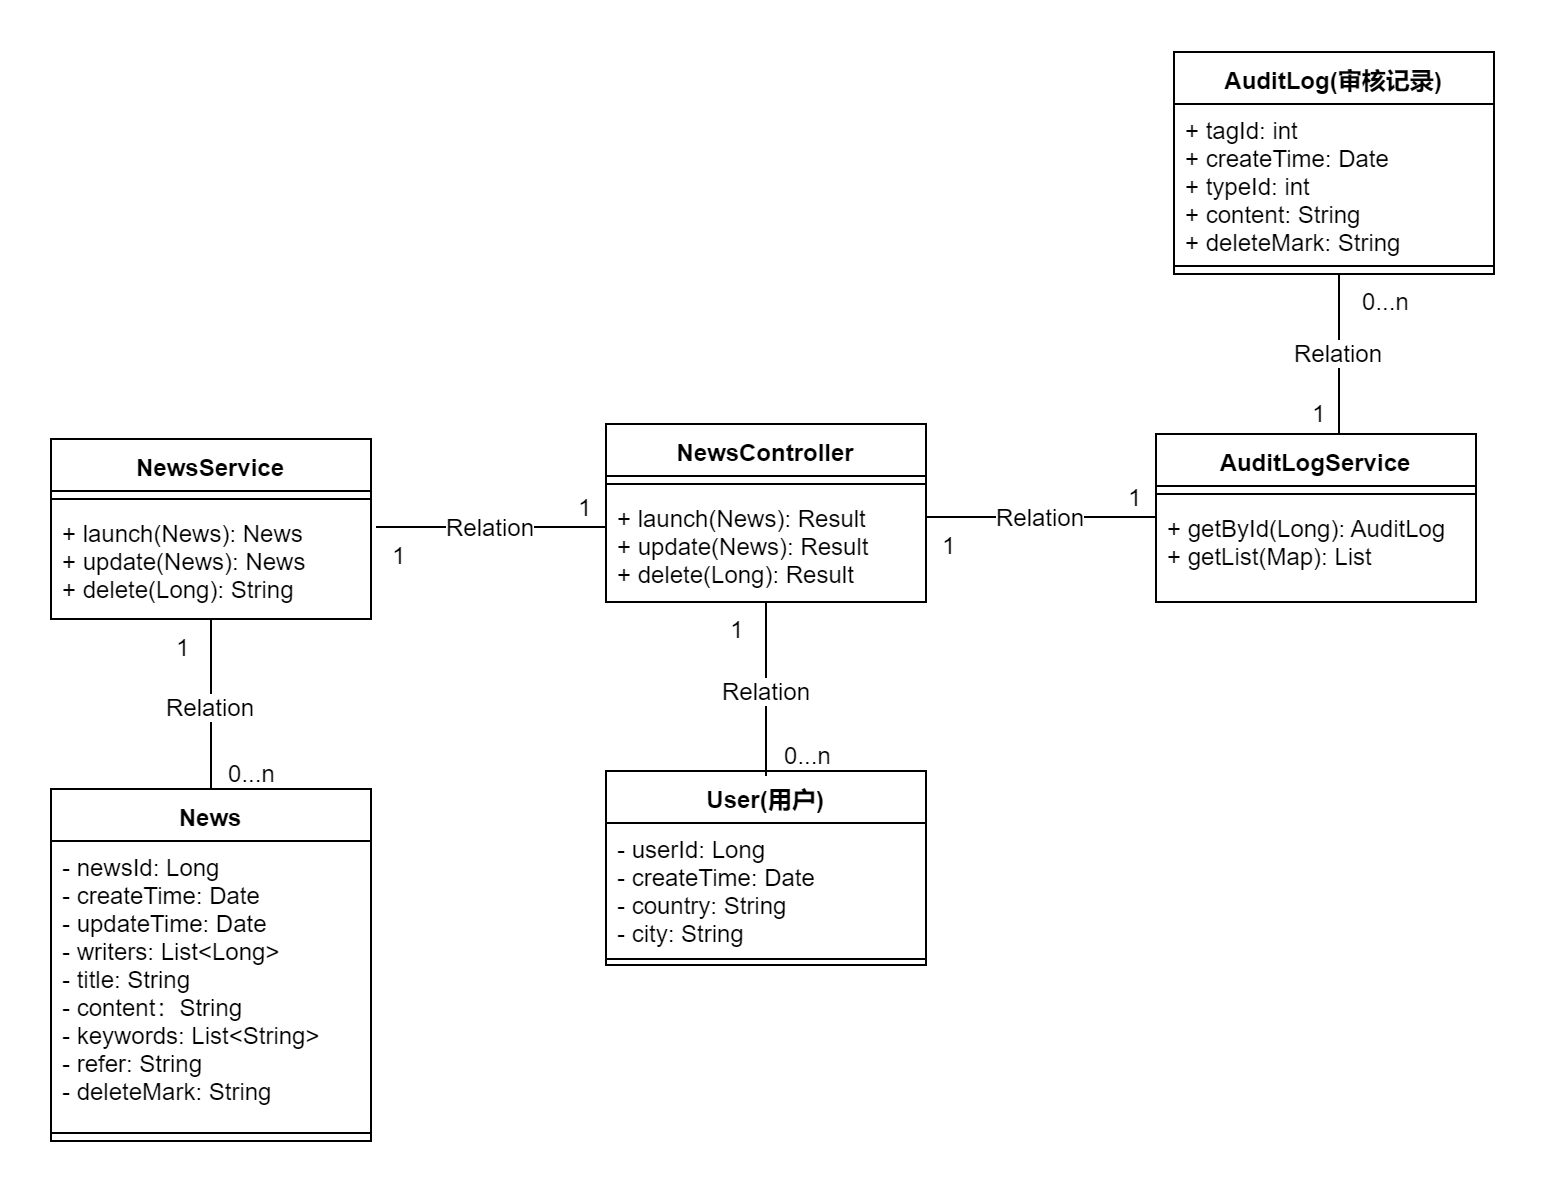
\includegraphics[width=1\textwidth]{ch5/LaunchNews.jpg}
    \caption{删除新闻}\label{fig:DeleteNews}
    \vspace{\baselineskip} % 表示图与正文空一行
\end{figure}
\section{举报}
所有用户都可以对新闻或者房源进行举报,举报需要填写举报理由,然后会由管理员进行审核,管理员会和被举报的用户进行交涉,若举报信息属实则下架发布信息。
涉及到的实体类有用户类(User),举报类(Report),审核类(AuditLog)。具体方法均在ReportController中进行调用。
\begin{figure}[htbp]
    \centering
    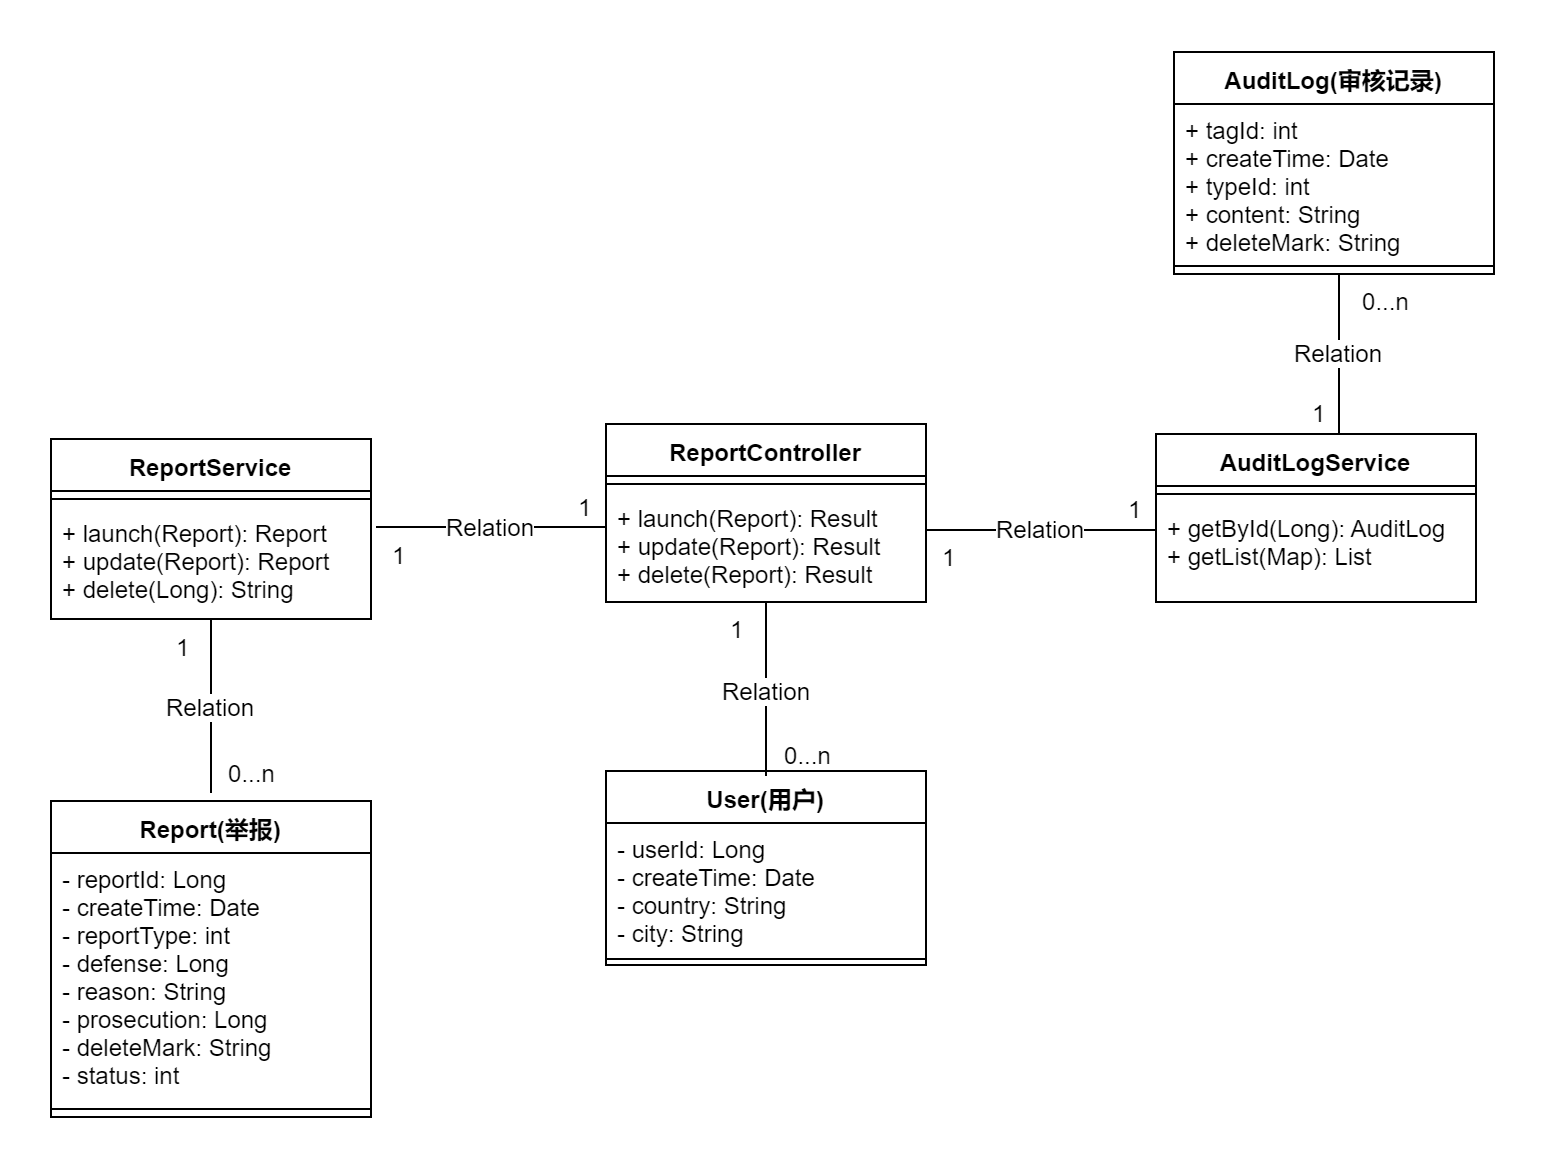
\includegraphics[width=1\textwidth]{ch5/Report.jpg}
    \caption{举报}\label{fig:Report}
    \vspace{\baselineskip} % 表示图与正文空一行
\end{figure}
\section{举报审核}
管理员对用户的举报进行审核,审核需要填写审核结果、审核信息,同时,还需要给涉及到的用户反馈审核结果,及通过系统通知反馈给举报人和被举报人,若举报人为
游客,则不予反馈。涉及到的实体类有用户类(User),举报类(Report),审核类(AuditLog),消息类(Message)。具体方法在AuditLogController中调用。
\begin{figure}[htbp]
    \centering
    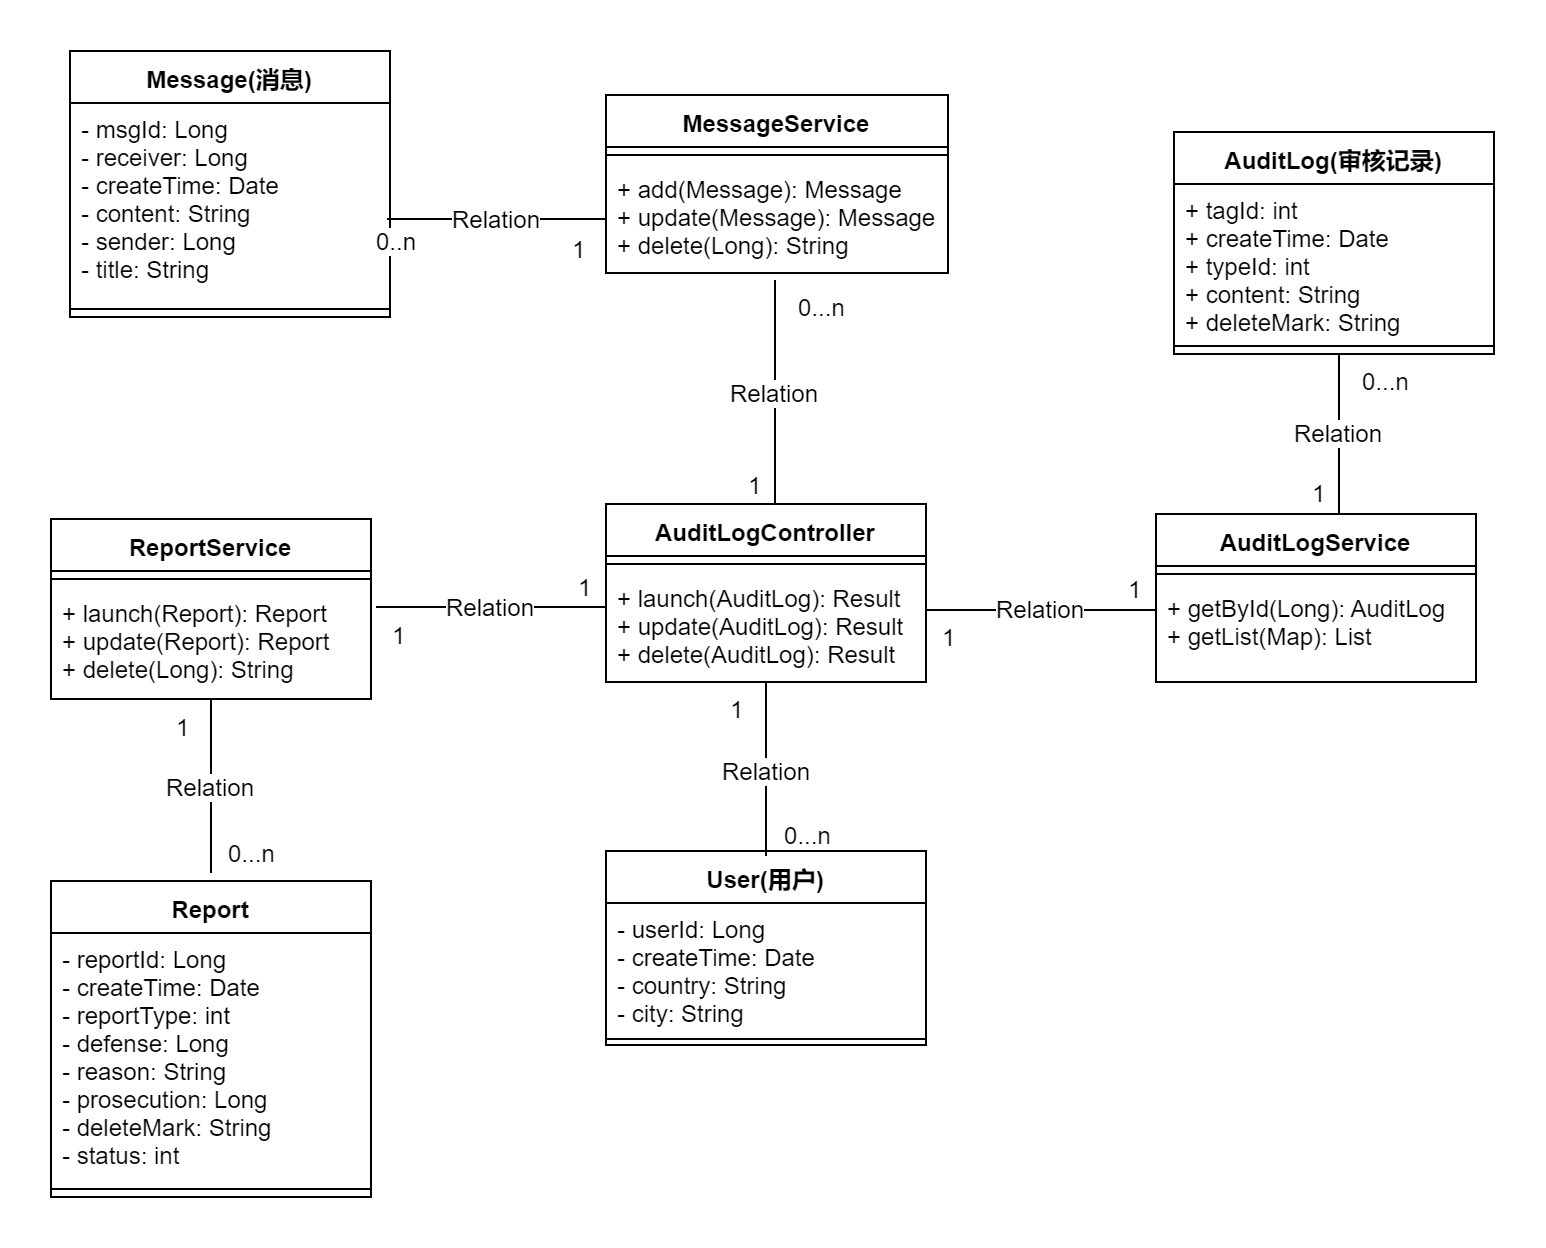
\includegraphics[width=1\textwidth]{ch5/AuditReport.jpg}
    \caption{举报审核}\label{fig:AuditReport}
    \vspace{\baselineskip} % 表示图与正文空一行
\end{figure}
\section{系统通知}
管理员通过消息的方式对用户进行系统通知,系统通知可以对全体用户广播,也可以针对于个别用户,管理员需要选择通知人群,填写通知内容。涉及到的实体类
有用户类(User),消息类(Message),具体方法在MessageController中调用。
\begin{figure}[htbp]
    \centering
    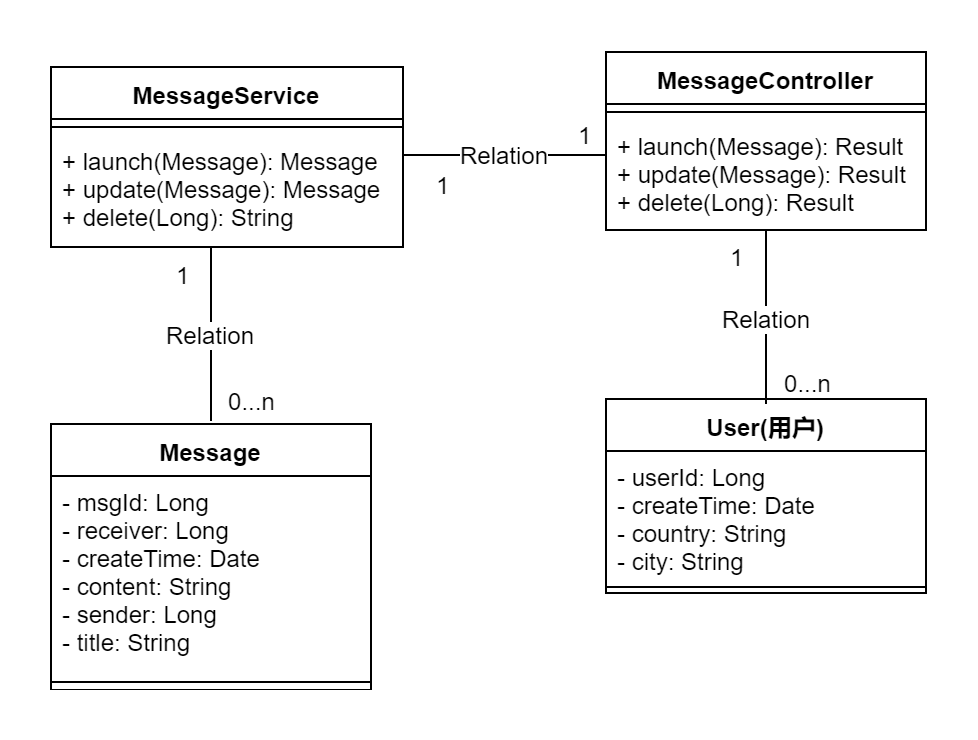
\includegraphics[width=1\textwidth]{ch5/Message.jpg}
    \caption{系统通知}\label{fig:Message}
    \vspace{\baselineskip} % 表示图与正文空一行
\end{figure}
\section{用户管理}
管理员可以通过后台对用户进行管理,包括用户封禁、用户查询、用户赋权、剥夺用户权限等操作,该模块的作用主要是对于用户权限的操作,涉及到的实体类有
用户类(User),角色类(Role),权限类(Permission)。涉及到的方法在UserController中进行调用。
\begin{figure}[htbp]
    \centering
    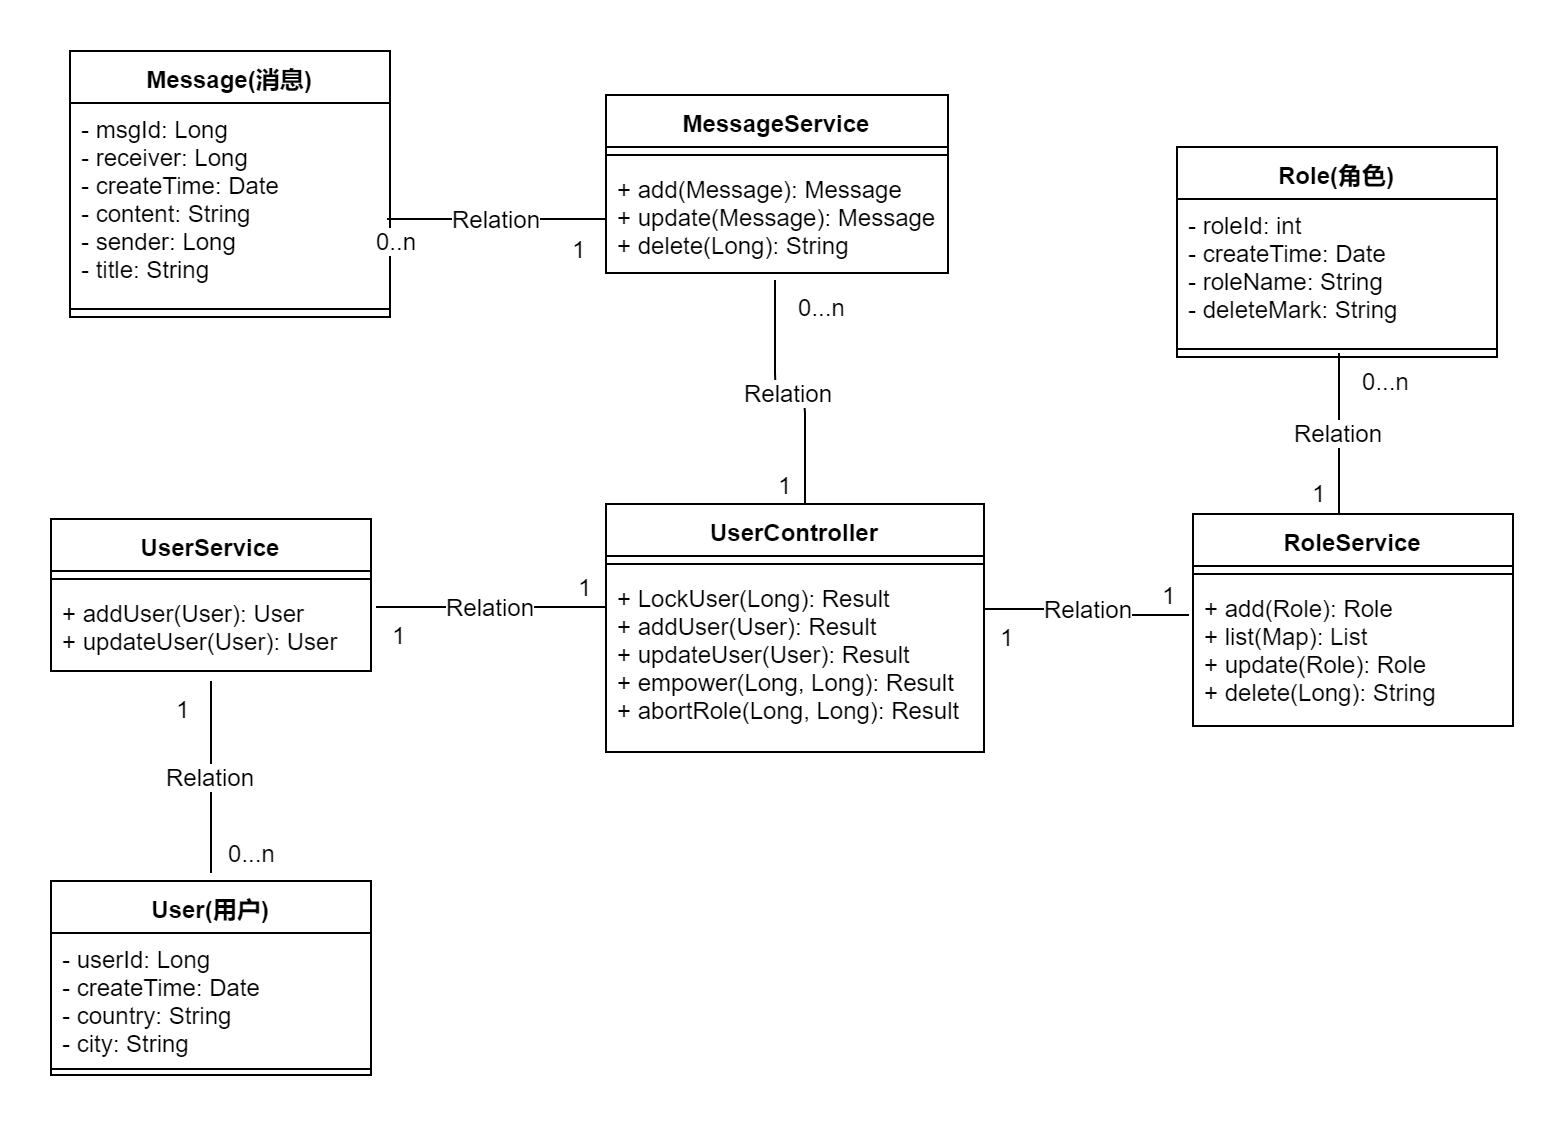
\includegraphics[width=1\textwidth]{ch5/UserManager.jpg}
    \caption{用户管理}\label{fig:UserManager}
    \vspace{\baselineskip} % 表示图与正文空一行
\end{figure}
\section{角色管理}
管理员可以通过后台对角色进行管理,包括删除角色,新增角色、角色赋权、剥夺角色权限等,该模块的作用主要是对于角色权限的操作,涉及到的实体类有
角色类(Role),权限类(Permission)。涉及到的方法在RoleController中进行调用。
\begin{figure}[htbp]
    \centering
    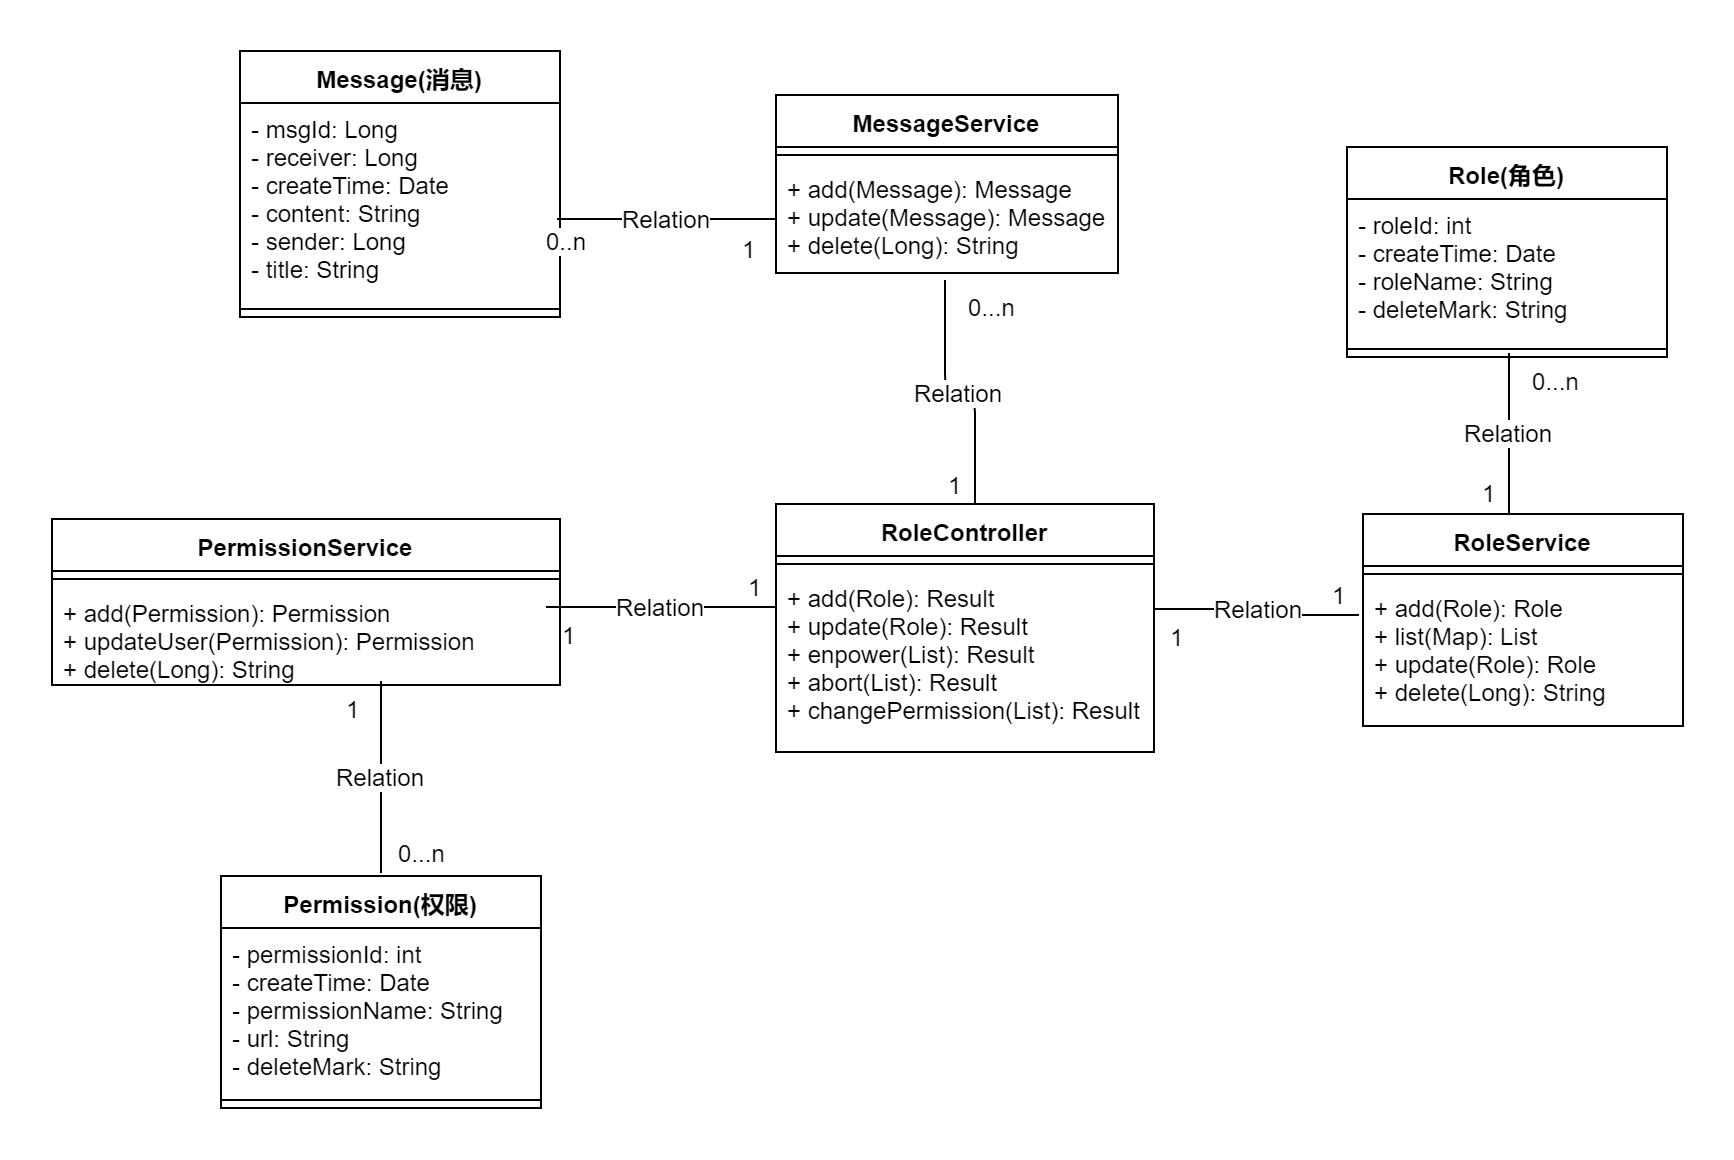
\includegraphics[width=1\textwidth]{ch5/RoleManager.jpg}
    \caption{角色管理}\label{fig:RoleManager}
    \vspace{\baselineskip} % 表示图与正文空一行
\end{figure}
\section{权限管理}
管理员可以通过后台对权限进行管理,包括删除权限,新增权限等,涉及到的实体类为权限类(Permission),方法均在PermissionController中调用。
\begin{figure}[htbp]
    \centering
    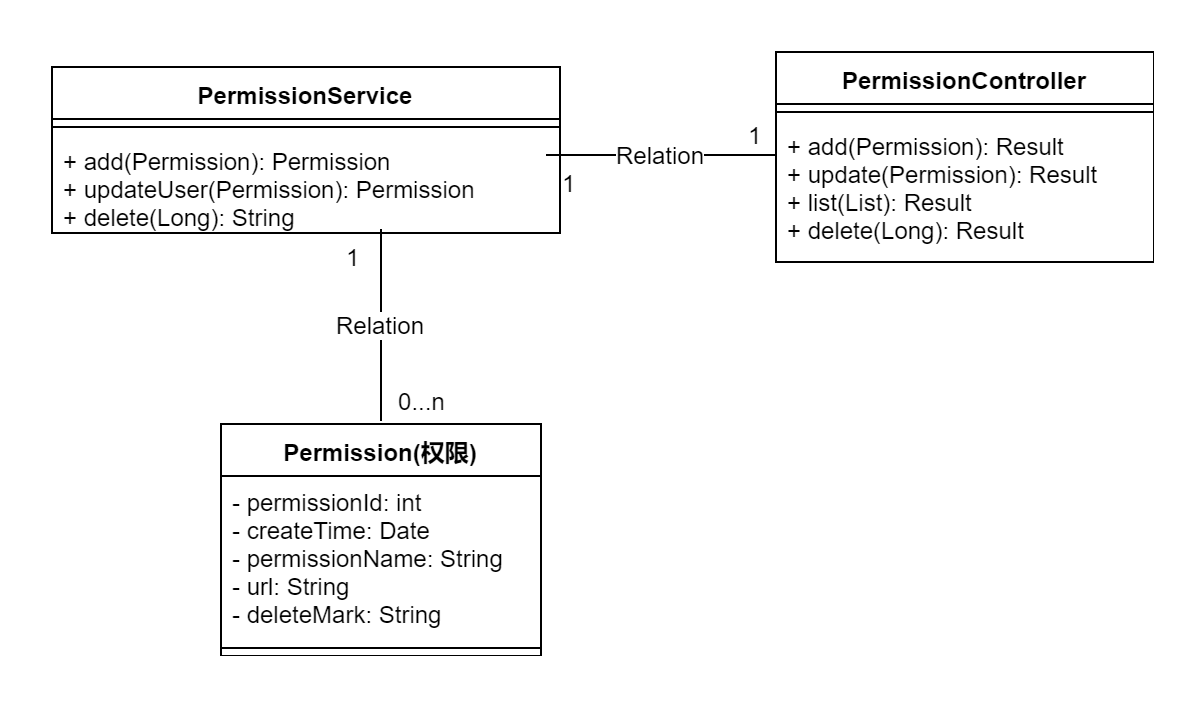
\includegraphics[width=1\textwidth]{ch5/PermissionManager.jpg}
    \caption{权限管理}\label{fig:PermissionManager}
    \vspace{\baselineskip} % 表示图与正文空一行
\end{figure}

